\documentclass{exam}
\usepackage{../../commonheader}

%%% CHANGE THESE %%%%%%%%%%%%%%%%%%%%%%%%%%%%%%%%%%%%%%%%%%%%%%%%%%%%%%%%%%%%%%
\discnumber{1}
\title{\textsc{Recursion and Higher Order Functions}}
\date{February 8 to February 12, 2016}
%%%%%%%%%%%%%%%%%%%%%%%%%%%%%%%%%%%%%%%%%%%%%%%%%%%%%%%%%%%%%%%%%%%%%%%%%%%%%%%

\begin{document}
\maketitle
\rule{\textwidth}{0.15em}
\fontsize{12}{15}\selectfont

%%% INCLUDE TOPICS HERE %%%%%%%%%%%%%%%%%%%%%%%%%%%%%%%%%%%%%%%%%%%%%%%%%%%%%%%

\section{Recursion}

Every Recursive function has three things.
\begin{enumerate}
\item One or more base cases
\item One or more ways to break the problem down into a smaller problem
\begin{itemize}
\item E.g. Given a number as input, we need to break it down into a smaller number
\end{itemize}
\item Solve the smaller problem recursively; from that, form a solution to the original problem
\end{enumerate}
\begin{questions}

%%% Question %%%

\begin{blocksection}
\question Write \texttt{numDigits}, which takes in a number \texttt{n} and returns the number of digits it has:

\begin{lstlisting}
def numDigits(n):
    """Takes in an positive integer and returns the number of digits

    >>> numDigits(0)
    0
    >>> numDigits(1)
    1
    >>> numDigits(7)
    1
    >>> numDigits(1093)
    4
    """
\end{lstlisting}

\begin{solution}[1in]
\begin{lstlisting}
 if n == 0:
   return 0
 else:
   return 1 + numDigits(n//10)
\end{lstlisting}
\end{solution}

\end{blocksection}

%%% Question %%%


\begin{blocksection}
\question Write a function \texttt{isSorted} that takes in an integer \texttt{n} and returns true if the digits of that number are increasing from right to left

\begin{lstlisting}
def isSorted(n): 
   """Return true if the digit is in increasing order from rightmost digit to leftmost digit. (Consecutive same digits are allowed). Also return true if it has only onedigit. Return false otherwise.
   >>> isSorted(2)
   True
   >>> isSorted(22222)
   True
   >>> isSorted(9876543210)
   True
   >>> isSorted(9087654321)
   False
   """
\end{lstlisting}

\begin{solution}[1in]
\begin{lstlisting}
right_digit = number % 10
rest =  number // 10
if rest  == 0:
    return True
elif right_digit > rest % 10 :
    return False
else:
  	return isSorted(rest) 
\end{lstlisting}
\end{solution}

\end{blocksection}

\section{Environment Diagrams}
\begin{blocksection}
\question Draw an environment diagram for the following code:

\begin{lstlisting}
x = 20
def foo(y):
    x = 5
    def bar():
        return lambda y: x-y
    return bar

y = foo(7)
z = y()
print(z(2))
\end{lstlisting}

\begin{solution}[2in] \newline
    Output: 3 \newline
    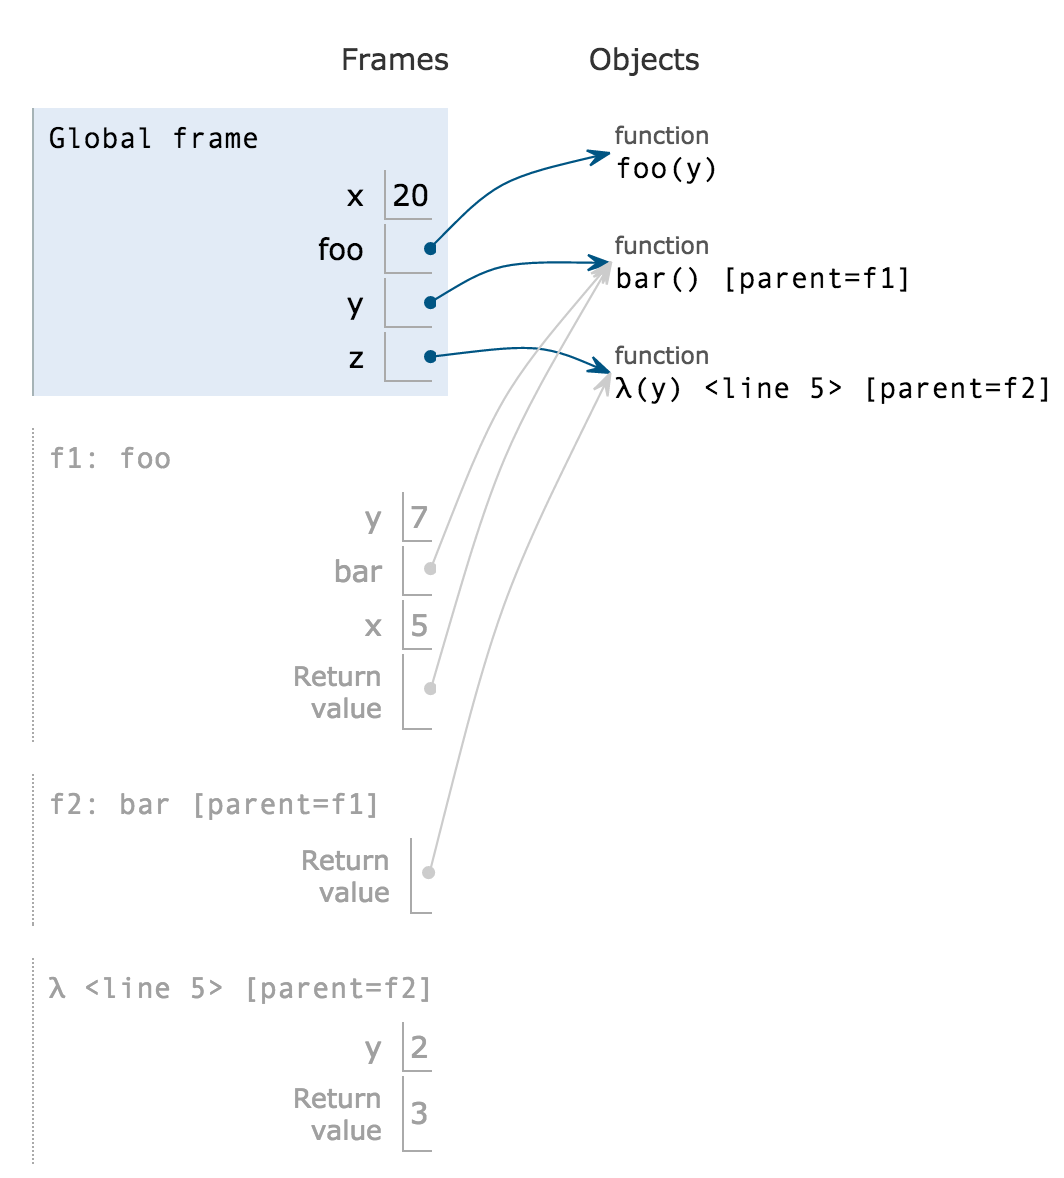
\includegraphics[scale=0.5]{img/foobar.png}
\end{solution}
\end{blocksection}

\begin{blocksection}
\question What would change here?

%% Prompt %%
\begin{lstlisting}
x = 20

def bar():
    return lambda y: x-y

def foo(y):
    x = 5
    return bar

y = foo(7)
z = y()
print(z(2))
\end{lstlisting}

\begin{solution}[0.3in] \newline
   Output: 18 \newline
    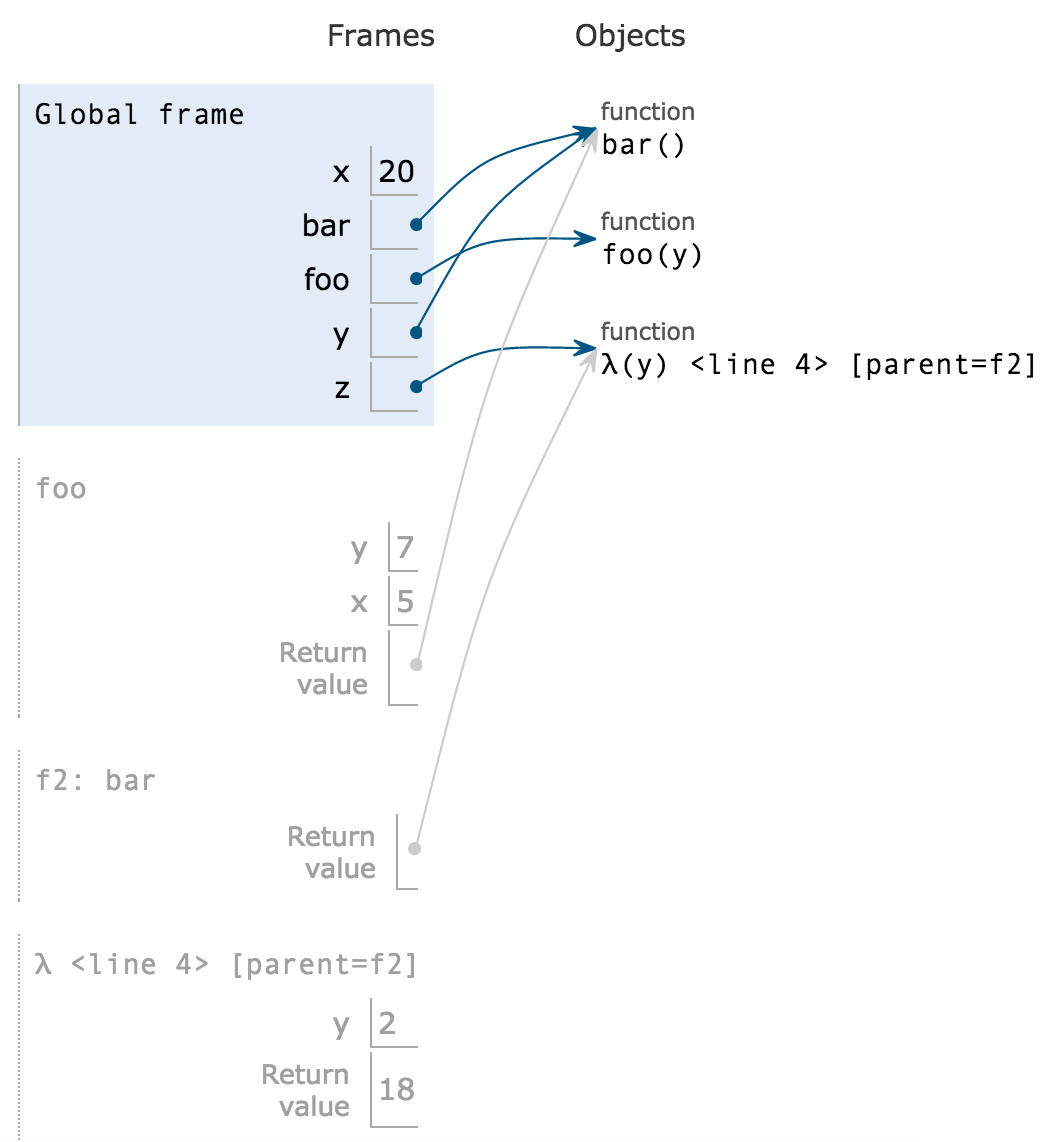
\includegraphics[scale=0.5]{img/foobar2.png}
\end{solution}
\end{blocksection}
\end{questions}

\section{Higher Order Functions}

\begin{questions}

%%% Question %%%

\begin{blocksection}
\question Write a higher order function that passes the following doctests. \emph{Challenge:} Write the function body in one line.

\begin{lstlisting}
"""
>>> from operator import add, mul
>>> a = mystery(add, 3)
>>> a(4) #equivalent to add(3,4)
7 
>>> a(12)
15
>>> b = mystery(mul, 5)
>>> b(7) #equivalent to mul(5,7)
35
>>> b(1)
5
>>> c = mystery(lambda x, y: x*x + y, 4)
>>> c(5)
21
>>> c(7)
23
"""
\end{lstlisting}

\begin{solution}[2in]
\begin{lstlisting}
def mystery(f, x):
	def helper(y):
		return f(x,y)
	return helper

One-line solution: return lambda y : f(x,y)
\end{lstlisting}
\end{solution}
\end{blocksection}

\question What do these print out?
\begin{lstlisting}
>>>foo = mystery(lambda a,b: a(b), lambda c: 5 + square(c))
>>>foo(-2)
\end{lstlisting}

\begin{solution}
9
\end{solution}

\end{questions}
%%%%%%%%%%%%%%%%%%%%%%%%%%%%%%%%%%%%%%%%%%%%%%%%%%%%%%%%%%%%%%%%%%%%%%%%%%%%%%%

\end{document}
